\documentclass{ximera}

%\addPrintStyle{../..}

\begin{document}
	\author{Bart Lambregs,Vincent Gellens}
	\xmtitle{De snelheid}{}
    \xmsource\xmuitleg


\sisetup{per-mode=symbol} %TEST VOOR DE SI EENHEDEN 

\NewDocumentCommand{\maakachtvar}{m m m m m m m m}{

\pgfmathsetmacro{\at}{#1}    \pgfmathsetmacro{\ax}{#2}
\pgfmathsetmacro{\bt}{#3}    \pgfmathsetmacro{\bx}{#4}
\pgfmathsetmacro{\ct}{#5}    \pgfmathsetmacro{\cx}{#6}
\pgfmathsetmacro{\dt}{#7}    \pgfmathsetmacro{\dx}{#8}

\pgfmathsetmacro{\tmin}{min(\at,\bt,\ct,\dt)}
\pgfmathsetmacro{\tmax}{max(\at,\bt,\ct,\dt)}
\pgfmathsetmacro{\xmin}{min(\ax,\bx,\cx,\dx)}
\pgfmathsetmacro{\xmax}{max(\ax,\bx,\cx,\dx)}

\pgfmathsetmacro{\deltat}{\tmax-\tmin}
\pgfmathsetmacro{\deltax}{\xmax-\xmin}

\pgfmathsetmacro{\xmargin}{0.08*\deltat}   
\pgfmathsetmacro{\ymargin}{0.3*\deltax} 

\pgfmathsetmacro{\xrangemin}{\tmin-\xmargin}
\pgfmathsetmacro{\xrangemax}{\tmax+\xmargin}
\pgfmathsetmacro{\yrangemin}{\xmin-\ymargin}
\pgfmathsetmacro{\yrangemax}{\xmax+\ymargin}
}


Een voorwerp in beweging heeft een snelheid. 
De ervaring leert dat hoe groter de snelheid, hoe groter de verplaatsing in een bepaald tijdsinterval. 
Als je fietst aan \SI{30}{\kilo\meter\per\hour}, leg je op één uur tijd \SI{30}{km} af. 
Als je wandelt aan \SI{5}{\kilo\meter\per\hour} leg je op één uur tijd slechts \SI{5}{km} af. 
De snelheid van een voorwerp kan volledig bepaald worden met behulp van de plaatsfunctie. 

We behandelen eerst de snelheid in één dimensie. 
Daarna kijken we naar de snelheid in twee dimensies, die wordt opgebouwd als samenstelling van twee (ééndimensionale) snelheidscomponenten. 


% Een voorwerp heeft snelheid als het beweegt, er is een verandering van de positie in de tijd.
% De snelheidsvector grijpt aan op het bewegend voorwerp en wijst in de zin van de ogenblikkelijke beweging, dat is rakend aan de baan dat het voorwerp maakt. % bewijs hiervoor van Bart kan toegevoegd worden
% In animaties lijkt het alsof de snelheidsvector aan de positievector 'trekt'. Bezie hiervoor animaties te vinden op https://www.hansbekaert.be/fysica/new/applets6.html.



\subsection*{Snelheid bij ééndimensionale bewegingen}

% gemiddelde snelheid als je een rondje loopt is nu nul; dat moet miss benoemd worden 

% Als een voorwerp op een rechte lijn beweegt (1D), dan valt de beweegrichting en dus ook die van de snelheidsvector samen met de richting van die lijn.  % dit weten ze nog niet...? 
% Bovenstaande zin is erg moeilijk; gemiddelde vector is eerder een scalar dan een vector. 

De tijd nodig voor een bepaalde verplaatsing geeft aanleiding tot de \textit{gemiddelde snelheid}. 

% hieronder gedefinieerd als een scalar --> niet helemeel eenduidig dus momenteel. 

\begin{definition}
	
In één dimensie wordt de gemiddelde snelheid $\overline{v}$ van een voorwerp tussen twee tijdstippen gedefiniëerd als
\[
\overline{v}=\frac{\Delta x}{\Delta t}=\frac{x_2-x_1}{t_2-t_1}
\]
De eenheid van snelheid is meter per seconde $[v]=\rm\,m/s$. 
\end{definition}


In het traject van de zeilboot is de gemiddelde snelheid van de boot tussen de tijdstippen $t_1$ en $t_2$ gelijk aan 
$\overline{v} =\frac{\Delta x}{\Delta t} =\frac{x_2-x_1}{t_2-t_1}=\frac{\SI{10}{\meter} - \SI{40}{\meter}}{\SI{15}{\second} - \SI{5}{\second}}= \frac{\SI{-30}{\meter}}{\SI{10}{\second}} = \SI{-3}{\meter\per\second}$. 
Deze gemiddelde snelheid is negatief, wat betekent dat de zeilboot tegen de positieve richting-as is bewogen. 


\begin{quickquestion*}{}{}
Kan je op de plaatsgrafiek van de zeilboot de gemiddelde snelheid tussen \(t_2\) en \(t_0\) aanduiden? 
\end{quickquestion*}



\subsection*{Ogenblikkelijke snelheid bij ééndimensionale bewegingen}

De gemiddelde snelheid \(\overline{v}\) is enkel gedefinieerd \textit{tussen} twee posities \(x_1\) en \(x_2\). 
De plaatsfunctie \(x(t)\) kent voor elk tijdstip \(t\) een positie \(x\) toe aan een puntmassa. Op dezelfde manier zou je op elk tijdstip de snelheid willen kennen. 

De eenheid van snelheid is \SI{}{\meter\per\second}, het gaat dus over het aantal meter dat in een bepaald tijds\-in\-ter\-val wordt afgelegd. 
Op één bepaald moment \(t\), één ogenblik, is er helemaal geen tijdsverloop en bijgevolg kan er ook geen verplaatsing zijn \ldots! Er is immers geen tijd verstreken om afstand te kunnen afleggen.

\begin{denkvraag*}{}
Als een raket opstijgt vanuit stilstand is de snelheid duidelijk groter dan nul. \textbf{Wat is volgens jou de snelheid op het eerste moment dat een opstijgende raket de grond niet meer raakt?}
\end{denkvraag*}


`Ja, maar', ga je zeggen, `de snelheidsmeter van mijn fiets zegt toch hoe hard ik ga?!' 
Dat \textit{lijkt} inderdaad een ogenblikkelijke snelheid te zijn maar in werkelijkheid is dat steeds de gemiddelde snelheid over het tijdsinterval dat het sensortje op je wiel nodig heeft om één omwenteling te maken. 
Je snelheidsmeter berekent dus de gemiddelde snelheid door je wielomtrek\footnote{Die je hebt moeten ingeven\ldots} te delen door de tijd van één omwenteling. 
Als je plots remt gaat je snelheid afnemen maar je metertje gaat dit niet ogenblikkelijk kunnen aangeven. 
Het moet wachten totdat het sensortje weer rond is geweest om de tijd te kennen en zo de snelheidsverandering te kunnen registreren.



% DIT GAAT WEL ALS DE TEKST INORDE IS
% % ------------------% % ------------------% % ------------------% % ------------------% % ------------------
% \begin{image}
% 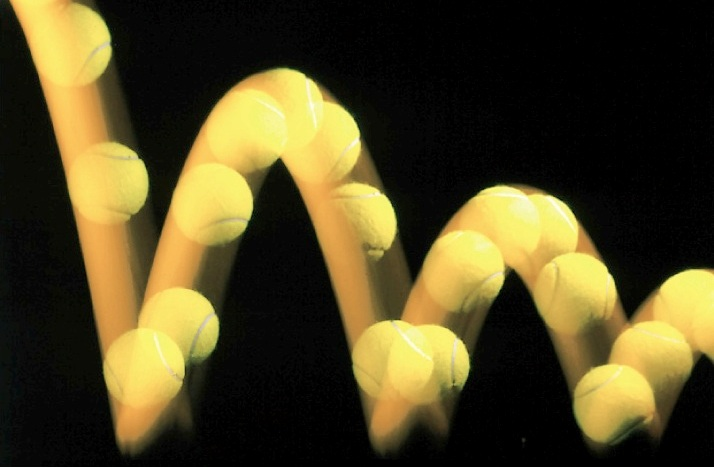
\includegraphics[width=0.8\textwidth]{stuiterendetennisbal}
% \end{image}
% \captionof{figure}{Stuiterende tennisbal}
% Hoe kan dit probleem opgelost worden? Op de stroboscopische foto van de stuiterende tennisbal is te zien dat de bal bovenaan trager beweegt dan wanneer hij de grond nadert. 
% Bovenaan liggen de beelden immers dichter bij elkaar zodat de tennisbal minder afstand aflegt in de tijdsspanne tussen twee opeenvolgende opnames. 
% Deze kwantitatieve\footnote{Kwantitatief wil zeggen dat het over een hoeveelheid of een grootte gaat.} informatie die levert echter opnieuw gemiddelde snelheid en niet zomaar de ogenblikkelijke snelheid. 
% De tennisbal verandert immers nog van snelheid tussen twee opeenvolgende opnames. 
% Door de frequentie\footnote{Frequentie is een grootheid die aangeeft hoeveel cyclussen er per seconde worden doorlopen. 
% Hier gaat het dus over het aantal beelden dat per seconde wordt gemaakt. 
% De eenheid van frequentie is $\rm\,s^{-1}$ oftewel Hz (de Hertz).} waarmee de foto's worden genomen op te drijven, krijgen we een accurater beeld van de snelheid die de tennisbal op een gegeven moment heeft. 
% De tijdsintervallen zijn nu immers korter zodat de bal minder van snelheid kan veranderen gedurende de intervallen en zodoende de gemiddelde snelheid een indicatie wordt van de ogenblikkelijke snelheid. 
% De ogenblikkelijke snelheid wordt dus beter en beter benaderd door het tijdsinterval kleiner en kleiner en kleiner en kleiner\ldots te nemen. Echter, hoe kort het tijdsinterval ook is, de snelheid zal veranderen gedurende dat hele kleine tijdsinterval.
% Daarom, je raadde het misschien al, wordt de ogenblikkelijke snelheid gedefinieerd als de \textit{limiet} van de gemiddelde snelheid over een tijdsinterval waarbij we dat interval naar nul laten gaan. 
% % ------------------% % ------------------% % ------------------% % ------------------% % ------------------


Hoe kan dit probleem opgelost worden? 
Om de ogenblikkelijke snelheid op \(t_1 = \SI{5}{\second}\) te kennen, lijk het eerste (en misschien wel enige...) idee om te vertrekken van de gemiddelde snelheid tussen \(t_1\) en \(t_2\) die hierboven werd berekend. 
Deze gemiddelde snelheid kan je beschouwen als een erg ruwe schatting van de snelheid op \(t_1 = 5\). 

\[
\overline{v} =\frac{\Delta x}{\Delta t} =\frac{x_2-x_1}{t_2-t_1}=\frac{\SI{10}{\meter} - \SI{40}{\meter}}{\SI{15}{\second} - \SI{5}{\second}}= \frac{\SI{-30}{\meter}}{\SI{10}{\second}} = \SI{-3}{\meter\per\second}
\] 


\maakachtvar{0}{30}{5}{40}{15}{10}{35}{-10}

\begin{image}[0.8\textwidth]
  \begin{tikzpicture}
  \begin{axis}[
	  axis x line=bottom,
	  axis y line=none,   
	  axis line style={->},
	  xmin= \yrangemin, xmax=\yrangemax,
	  ymin=-1, ymax=3,  %plek voor schepen en tijdlabels 
	  xlabel={Positie--as (in meter)},
	  xtick distance=5,
	  xticklabel={\tiny\SI[round-precision=0, round-mode=places]{\tick}{m}},
	  width=14cm, height=4cm,
  ]

  % Schip niet tonen-->opacity op nul
  \node[opacity=0,scale=1,xscale=-1]  (schip0) at (axis cs:\ax,0.5)  {
\includegraphics[width=1cm]{schip_icoon}};
  \node[opacity=0,draw, rectangle, inner sep=1pt] (t1) at (axis cs:\ax,2.2) {\small $t_0=\SI{\at}{\second}$};

  \node[opacity=1,scale=1,xscale=1] (schip1) at (axis cs:\bx,0.5)  {
\includegraphics[width=1cm]{schip_icoon}};
  \node[draw, rectangle, inner sep=1pt] (t2) at (axis cs:\bx,2.2) {\small $t_1=\SI{\bt}{\second}$};

  \node[opacity=1]                     (schip2) at (axis cs:\cx,0.5) {
\includegraphics[width=1cm]{schip_icoon}};
  \node[draw, rectangle, inner sep=1pt] (t3) at (axis cs:\cx,2.2) {\small $t_2=\SI{\ct}{\second}$};

  % Schip niet tonen-->opacity op nul
  \node[opacity=0]                                (schip3) at (axis cs:\dx,0.5) {
\includegraphics[width=1cm]{schip_icoon}};
  \node[opacity=0, draw, rectangle, inner sep=1pt] (t4) at (axis cs:\dx,2.2) {\small $t_3=\SI{\dt}{\second}$};

  \draw[<->, dotted, red] (schip1) -- (schip2) node[midway, fill=white]{\(\Delta x\)};

  
  \end{axis}
  \end{tikzpicture}

  \begin{tikzpicture}
  \begin{axis}[
	  axis x line=bottom,
	  axis y line=left,
	  axis line style={->},
	  xlabel={tijd (in seconden)},
	  ylabel={positie (in meter)},
	  xmin= \xrangemin, xmax=\xrangemax,
	  ymin= \yrangemin, ymax=\yrangemax,
	  xtick distance=5,
	  ytick distance=10,
	  xticklabel={\SI[round-precision=0, round-mode=places]{\tick}{s}},
	  yticklabel={\SI[round-precision=0, round-mode=places]{\tick}{m}},
	  grid=both,
	  width=15cm, height=10cm,
  ]

  \addplot[blue, thick, smooth, tension=0.5] coordinates{
	  (\at,\ax)
	  (\bt,\bx)
	  (\ct,\cx)
	  (\dt,\dx)
  };
  
  % SCHIP NIET AFBEELDEN --> OPACITY 0 
  \node[opacity=0] (schip0) at (axis cs:\at,\ax) {
\includegraphics[width=1cm]{schip_icoon}};
  \node[opacity=0, draw, rectangle, inner sep=1pt] at (axis cs:\at,\ax+10) {\small $t_0=\SI{\at}{\second}$};

  \node[] (schip1) at (axis cs:\bt,\bx) {
\includegraphics[width=1cm]{schip_icoon}};
  \node[draw, rectangle, inner sep=1pt] at (axis cs:\bt,\bx+10) {\small $t_1=\SI{\bt}{\second}$};

  \node[] (schip2) at (axis cs:\ct,\cx) {
\includegraphics[width=1cm]{schip_icoon}};
  \node[draw, rectangle, inner sep=1pt] at (axis cs:\ct,\cx+10) {\small $t_2=\SI{\ct}{\second}$};

  % SCHIP NIET AFBEELDEN --> OPACITY 0 
  \node[opacity=0] (schip3) at (axis cs:\dt,\dx) {
\includegraphics[width=1cm]{schip_icoon}};
  \node[opacity=0, draw, rectangle, inner sep=1pt] at (axis cs:\dt,\dx+10) {\small $t_3=\SI{\dt}{\second}$};

  % --- DeltaX accolade ---
  \draw[decorate, decoration={brace, amplitude=5pt, mirror}, red, thick] 
  (axis cs:\bt,\bx) -- (axis cs:\bt,\cx) 
  node[midway, left, xshift=-4pt] {\small $\Delta x$};

  % --- DeltaT accolade ---
  \draw[decorate, decoration={brace, amplitude=5pt, mirror}, xmgreen, thick] 
	  (axis cs:\bt,\cx) -- (axis cs:\ct,\cx) 
	  node[midway, below, yshift=-2pt] {\small $\Delta t$};

  \end{axis}
  \end{tikzpicture}
\end{image}
\captionof{figure}{De gemiddelde snelheid voor \(t_1 = 5\) en \(t_3 = 15\)}

Indien niet met \(t_2 = 15\) de gemiddelde snelheid wordt berekent, maar bijvoorbeeld met \(t_l = \SI{10}{\second} \), zal deze gemiddelde snelheid beter de ogenblikkelijke snelheid op \(t_1\) benaderen. 

% Op de grafiek zien we dat \(x_l = 22\) en een rechtsreekse berekening levert dan dat de gemiddelde snelheid tussen \(t_1=5\) en \(t_l=8\) gegeven wordt door 

% \[
% \overline{v}=\frac{x_l-x_1}{t_l-t_1}=\frac{\SI{22}{\meter} - \SI{40}{\meter}}{\SI{10}{\second} - \SI{5}{\second}}=  \frac{\SI{-18}{\meter}}{\SI{5}{\second}} = \SI{-3.6}{\meter\per\second}
% \]

De gemiddelde snelheid is kleiner geworden en op de plaatsgrafiek schuift de zeilboot in de richting van \(t_1\). 
De gemiddelde snelheid \(\bar{v} = \frac{x_l - x_1}{t_l-t_1}\) is een \textit{betere} benadering voor de ogenblikkelijke snelheid op \(t_a\). 
Maar het is nog steeds een gemiddelde snelheid! 
De lezer raadde het waarschijnlijk al...

Door de gemiddelde snelheid te berekenen voor \(t_m = 7\) wordt de benadering voor de ogenblikkelijke snelheid op \(t_1\) nog beter... 
Op de grafiek komen de twee schepen nu wel erg dicht bij elkaar... 

% \[
% \overline{v}=\frac{x_2-x_m}{t_2-t_m}=\frac{\SI{31}{\meter} - \SI{40}{\meter}}{\SI{7}{\second} - \SI{5}{\second}}=  \frac{\SI{9}{\meter}}{\SI{2}{\meter}} = \SI{4.5}{\meter\per\second}
% \]

% HIER ZIJN DE NUMMER NOG FOUT --> WORDT GROTER DOOR AFRONDINGSFOUTEN... 

\maakachtvar{0}{30}{5}{40}{15}{10}{35}{-10}

\begin{image}[0.8\textwidth]
  \begin{tikzpicture}
  \begin{axis}[
	  axis x line=bottom,
	  axis y line=none,   
	  axis line style={->},
	  xmin= \yrangemin, xmax=\yrangemax,
	  ymin=-1, ymax=3,  %plek voor schepen en tijdlabels 
	  xlabel={Positie--as (in meter)},
	  xtick distance=5,
	  xticklabel={\tiny\SI[round-precision=0, round-mode=places]{\tick}{m}},
	  width=14cm, height=4cm,
  ]

  % Schip niet tonen-->opacity op nul
  \node[opacity=0,scale=1,xscale=-1]  (schip0) at (axis cs:\ax,0.5)  {
\includegraphics[width=1cm]{schip_icoon}};
  \node[opacity=0,draw, rectangle, inner sep=1pt] (t1) at (axis cs:\ax,2.2) {\small $t_0=\SI{\at}{\second}$};

  \node[opacity=1,scale=1,xscale=1] (schip1) at (axis cs:\bx,0.5)  {
\includegraphics[width=1cm]{schip_icoon}};
  \node[draw, rectangle, inner sep=1pt] (t2) at (axis cs:\bx,2.2) {\small $t_1=\SI{\bt}{\second}$};

  \node[opacity=1]                     (schip2) at (axis cs:\cx,0.5) {
\includegraphics[width=1cm]{schip_icoon}};
  \node[draw, rectangle, inner sep=1pt] (t3) at (axis cs:\cx,2.2) {\small $t_2=\SI{\ct}{\second}$};

  \node[opacity=1]                     (schipl) at (axis cs:22,0.5) {
\includegraphics[width=1cm]{schip_icoon}};
  \node[draw, rectangle, inner sep=1pt] (t3) at (axis cs:22,2.2) {\small $t_l=\SI{10}{\second}$};

  \node[opacity=1]                     (schipm) at (axis cs:31,0.5) {
\includegraphics[width=1cm]{schip_icoon}};
  \node[draw, rectangle, inner sep=1pt] (t3) at (axis cs:31,2.2) {\small $t_m=\SI{7}{\second}$};

  % Schip niet tonen-->opacity op nul
  \node[opacity=0]                                (schip3) at (axis cs:\dx,0.5) {
\includegraphics[width=1cm]{schip_icoon}};
  \node[opacity=0, draw, rectangle, inner sep=1pt] (t4) at (axis cs:\dx,2.2) {\small $t_3=\SI{\dt}{\second}$};

%   \draw[<->, dotted, red] (schip1) -- (schipm) node[above, fill=white]{\(\Delta x\)};

  
  \end{axis}
  \end{tikzpicture}

  \begin{tikzpicture}
  \begin{axis}[
	  axis x line=bottom,
	  axis y line=left,
	  axis line style={->},
	  xlabel={tijd (in seconden)},
	  ylabel={positie (in meter)},
	  xmin= \xrangemin, xmax=\xrangemax,
	  ymin= \yrangemin, ymax=\yrangemax,
	  xtick distance=5,
	  ytick distance=10,
	  xticklabel={\SI[round-precision=0, round-mode=places]{\tick}{s}},
	  yticklabel={\SI[round-precision=0, round-mode=places]{\tick}{m}},
	  grid=both,
	  width=15cm, height=10cm,
  ]

  \addplot[blue, thick, smooth, tension=0.5] coordinates{
	  (\at,\ax)
	  (\bt,\bx)
	  (\ct,\cx)
	  (\dt,\dx)
  };
  
  % SCHIP NIET AFBEELDEN --> OPACITY 0 
  \node[opacity=0] (schip0) at (axis cs:\at,\ax) {
\includegraphics[width=1cm]{schip_icoon}};
  \node[opacity=0, draw, rectangle, inner sep=1pt] at (axis cs:\at,\ax+10) {\small $t_0=\SI{\at}{\second}$};

  \node[] (schip1) at (axis cs:\bt,\bx) {
\includegraphics[width=1cm]{schip_icoon}};
  \node[draw, rectangle, inner sep=1pt] at (axis cs:\bt,\bx+10) {\small $t_1=\SI{\bt}{\second}$};

  \node[] (schip2) at (axis cs:\ct,\cx) {
\includegraphics[width=1cm]{schip_icoon}};
  \node[draw, rectangle, inner sep=1pt] at (axis cs:\ct,\cx+10) {\small $t_2=\SI{\ct}{\second}$};

  \node[] (schipl) at (axis cs:10,22) {
\includegraphics[width=1cm]{schip_icoon}};
  \node[draw, rectangle, inner sep=1pt] at (axis cs:10,22+10) {\small $t_l=\SI{10}{\second}$};

  \node[] (schipm) at (axis cs:7,31) {
\includegraphics[width=1cm]{schip_icoon}};
  \node[draw, rectangle, inner sep=1pt] at (axis cs:8,31+10) {\small $t_m=\SI{7}{\second}$};

  % SCHIP NIET AFBEELDEN --> OPACITY 0 
  \node[opacity=0] (schip3) at (axis cs:\dt,\dx) {
\includegraphics[width=1cm]{schip_icoon}};
  \node[opacity=0, draw, rectangle, inner sep=1pt] at (axis cs:\dt,\dx+10) {\small $t_3=\SI{\dt}{\second}$};

  % --- DeltaX accolade ---
  \draw[decorate, decoration={brace, amplitude=5pt, mirror}, red, thick] 
  (axis cs:\bt,\bx) -- (axis cs:\bt,22) 
  node[midway, left, xshift=-4pt] {\small $\Delta x$};

  % --- DeltaT accolade ---
  \draw[decorate, decoration={brace, amplitude=5pt, mirror}, xmgreen, thick] 
	  (axis cs:\bt,22) -- (axis cs:10,22) 
	  node[midway, below, yshift=-2pt] {\small $\Delta t$};

  \end{axis}
  \end{tikzpicture}
\end{image}
\captionof{figure}{De gemiddelde snelheid voor \(t_1 = 5\) en \(t_l = 10\)}







De ogenblikkelijke snelheid wordt dus beter en beter benaderd door het tijdsinterval kleiner en kleiner en kleiner en kleiner\ldots te nemen. 
Echter, hoe kort het tijdsinterval ook is, de snelheid zal veranderen gedurende dat hele kleine tijdsinterval.
Daarom wordt de ogenblikkelijke snelheid gedefinieerd als de \textbf{limiet van de gemiddelde snelheid} over een tijdsinterval waarbij we dat interval naar nul laten gaan. 

\begin{definition}
	
De \textbf{ogenblikkelijke snelheid}  in één dimensie is de afgeleide van de plaatsfunctie:
\[
v=\lim_{\Delta t\to 0}\frac{\Delta x}{\Delta t}=\lim_{t\to t_0}\frac{x(t)-x(t_0)}{t-t_0}=\frac{dx}{dt}
\]
De notatie met een accent $v(t)=x'(t)$ of $v=x'$ wordt op dezelfde manier als in de wiskunde gebruikt. 
De functie $v(t)$ geeft op elk moment $t$ de snelheid $v(t)$. 
\end{definition}


Grafisch kan je de afgeleide terugvinden als de richtingscoöefficiënt van de raaklijn. In een $x-t$ grafiek (de grafiek van de functie $x(t)$, $x$ in functie van $t$) vind je de snelheid als de richtingscoöefficiënt van de raaklijn in het beschouwde punt. 

\begin{image}[0.4\textwidth]
	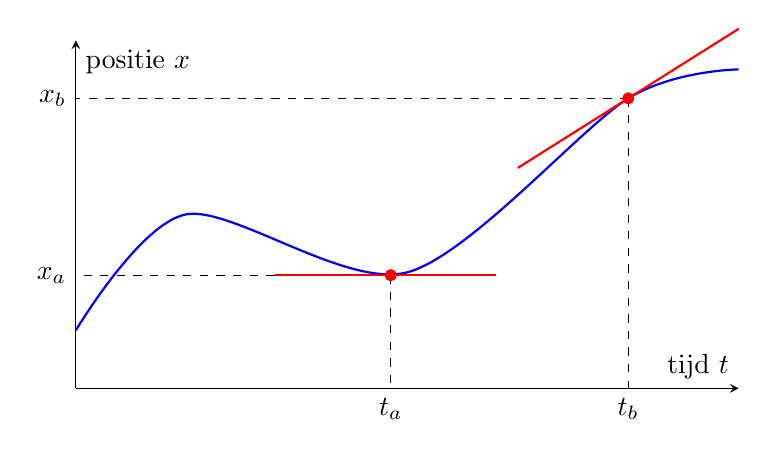
\begin{tikzpicture}
		\begin{axis}[
			axis lines=middle,
			xlabel={tijd \(t\)}, ylabel={positie \(x\)},
			grid=both,
			width=10cm, height=6cm,
			xmin=0, xmax=6, ymin=0, ymax=6,
			xtick=\empty,
			ytick=\empty,
			clip=false,
		]
		% Keep original curve
		\addplot[
			smooth,
			thick,
			color=blue
		] coordinates {
			(0,1) (1,3) (3,2) (5,5) (6,5.5)
		};

		% Red points (only moved t_a dot)
		\addplot[
			only marks,
			mark=*,
			mark size=2pt,
			color=red
		] coordinates {
			(2.85,1.95) (5,5)
		};

		% Dashed guide lines
		\draw[dashed] (axis cs:2.85,1.95) -- (axis cs:2.85,0) node[below]{$t_a$};
		\draw[dashed] (axis cs:2.85,1.95) -- (axis cs:0,1.95) node[left]{$x_a$};
		\draw[dashed] (axis cs:5,5) -- (axis cs:5,0) node[below]{$t_b$};
		\draw[dashed] (axis cs:5,5) -- (axis cs:0,5) node[left]{$x_b$};

		% Tangent lines
		\addplot[domain=1.8:3.8, thick, color=red] 
			{0*(x-2.85) + 1.95};  % horizontal tangent through new red dot
		\addplot[domain=4:6, thick, color=red] 
			{1.2*(x-5) + 5};
		\end{axis}
	\end{tikzpicture}
\end{image}
\captionof{figure}{De snelheid als rico aan de raaklijn}


\begin{definition}
De \textbf{snelheidsfunctie} \(\vec{v}(t)\) geeft voor elke moment \(t\) de snelheidsvector \(\vec{v}\). \\
In één dimensie is \(\vec{v}\) een scalar en is de plaatsfuncie een grafiek waarop horizontaal de tijd wordt weergegeven en verticaal de grootte van de snelheid. 
De snelheid op een welbepaald tijdstip \(t_a\) wordt genoteerd als 
\[
v_a = v(t_a)
\]

\begin{image}[0.4\textwidth]
	\begin{tikzpicture}
		\begin{axis}[
			axis lines=middle,
			xlabel={tijd \(t\)}, ylabel={snelheid \(v\)},
			grid=both,
			width=10cm, height=6cm,
			xmin=0, xmax=6, ymin=-1, ymax=3,
			xtick=\empty,
			ytick=\empty,
			clip=false,
		]

		% Red points for t_a and t_b
		\addplot[
			only marks,
			mark=*,
			mark size=2pt,
			color=red
		] coordinates {
			(2.85,0) (5,1.2)
		};

		% Dashed guide lines
		\draw[dashed] (axis cs:2.85,0) -- (axis cs:2.85,0) node[below]{$t_a$};
		\draw[dashed] (axis cs:2.85,0) -- (axis cs:0,0) node[left]{$v_a$};
		\draw[dashed] (axis cs:5,1.2) -- (axis cs:5,0) node[below]{$t_b$};
		\draw[dashed] (axis cs:5,1.2) -- (axis cs:0,1.2) node[left]{$v_b$};

		% Smooth velocity curve (updated with zero at t_a=2.85)
		\addplot[
			smooth,
			thick,
			color=blue
		] coordinates {
			(0,1) (1,0) (2,-0.6) (2.85,0) (4,1) (5,1.2) (6,0.5)
		};
	
		\end{axis}
	\end{tikzpicture}
\end{image}
\captionof{figure}{Een snelheidsfunctie voor een ééndimensionale beweging.}


\end{definition}



% dit zit in tikz nu
% \begin{image}
% 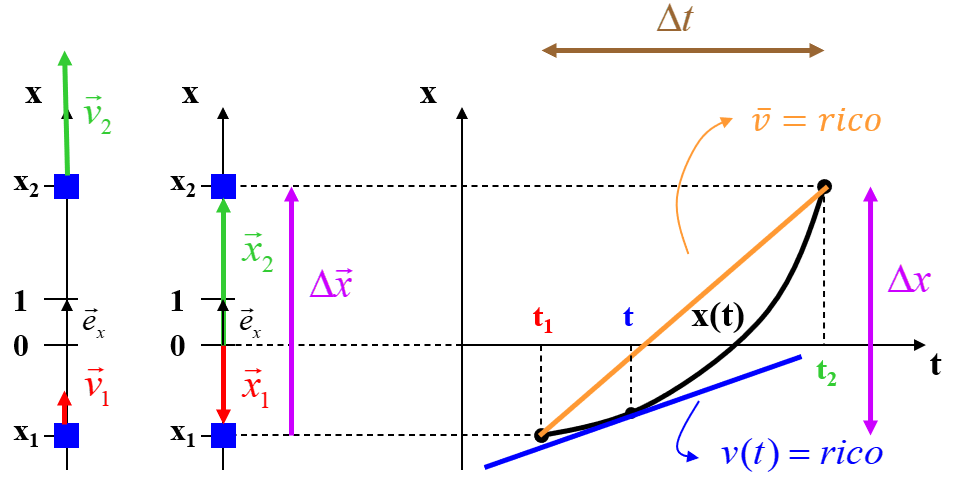
\includegraphics[width=0.8\textwidth]{snelheid1D}

% \end{image}

% \begin{image}
% 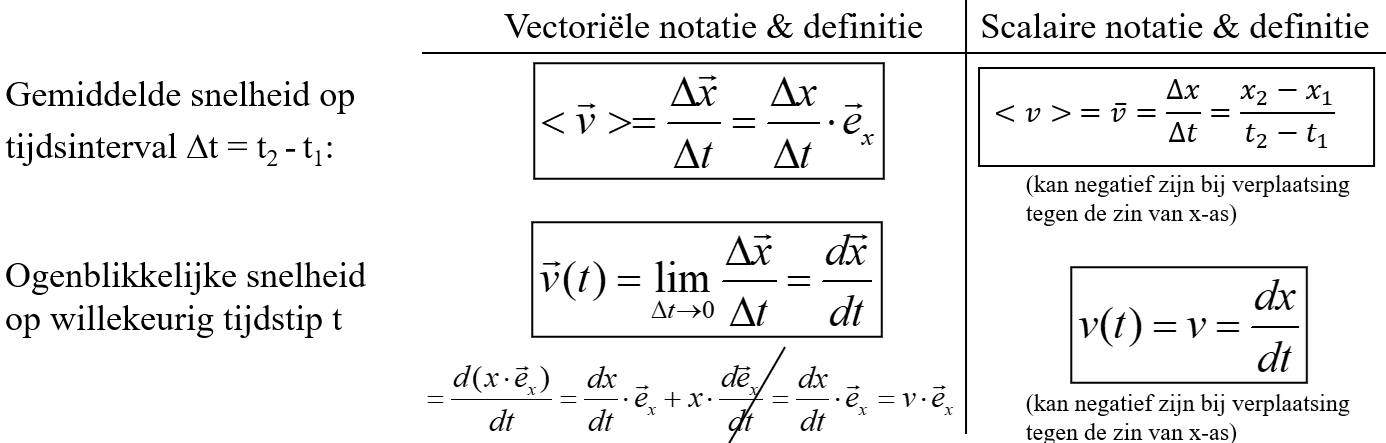
\includegraphics[width=0.8\textwidth]{overzichtsnelheid1D}

% \end{image}


% DIT IS NOG NIET GOED --> IS GEWOON OM GEEN SCREENSHOTS MEER IN DE CURSUS TE HEBBEN...! 

% \textbf{Gemiddelde snelheid op tijdsinterval } $\Delta t = t_2 - t_1$:
% \[
% \text{Vectoriële notatie: } \quad
% \langle \vec{v} \rangle = \frac{\Delta \vec{x}}{\Delta t} = \frac{\Delta x}{\Delta t} \cdot \vec{e}_x
% \]
% \[
% \text{Scalaire notatie: } \quad
% \langle v \rangle = \bar{v} = \frac{\Delta x}{\Delta t} = \frac{x_2 - x_1}{t_2 - t_1} 
% \quad \text{(kan negatief zijn bij verplaatsing tegen de zin van de x-as)}
% \]

% \textbf{Ogenblikkelijke snelheid op willekeurig tijdstip } $t$:
% \[
% \text{Vectoriële notatie: } \quad
% \vec{v}(t) = \lim_{\Delta t \to 0} \frac{\Delta \vec{x}}{\Delta t} = \frac{d\vec{x}}{dt} 
% = \frac{d(x \cdot \vec{e}_x)}{dt} = \frac{dx}{dt} \cdot \vec{e}_x + x \cdot \frac{d\vec{e}_x}{dt} = \frac{dx}{dt} \cdot \vec{e}_x = v \cdot \vec{e}_x
% \]
% \[
% \text{Scalaire notatie: } \quad
% v(t) = v = \frac{dx}{dt} \quad \text{(kan negatief zijn bij verplaatsing tegen de zin van de x-as)}
% \]


\begin{remark}
	Het woord 'ogenblikkelijk' mag je weglaten. Wanneer we het over snelheid hebben, bedoelen we vanaf nu steeds ogenblikkelijke snelheid.
\end{remark}



\begin{exercise}
Hieronder staat opnieuw de plaatsfunctie \(x(t)\) van de zeilboot. Bepaal enkel met de grafiek en zonder te rekenen: 
\begin{question} Waar ligt de zeilboot stil?                    \end{question}
\begin{question} Waar heeft de zeilboot een positieve snelheid? \end{question}
\begin{question} waar is de snelheid negatief?                  \end{question}
\begin{question} Op welk moment bewoog de zeilboot het snelst?  \end{question}

\begin{image}[0.5\textwidth]
	\begin{tikzpicture}
		\begin{axis}[
			axis x line=bottom,
			axis y line=left,
			axis line style={->},
			xlabel={tijd (in seconden)},
			ylabel={positie (in meter)},
			xmin= \xrangemin, xmax=\xrangemax,
			ymin= \yrangemin, ymax=\yrangemax,
			xtick distance=5,
			ytick distance=10,
			xticklabel={\SI[round-precision=0, round-mode=places]{\tick}{s}},
			yticklabel={\SI[round-precision=0, round-mode=places]{\tick}{m}},
			grid=both,
			width=15cm, height=10cm,
		]

		\addplot[blue, thick, smooth, tension=0.5] coordinates{
			(\at,\ax)
			(\bt,\bx)
			(\ct,\cx)
			(\dt,\dx)
		};
		
		\node[] at (axis cs:\at,\ax) {
\includegraphics[width=1cm]{schip_icoon}};
		\node[draw, rectangle, inner sep=1pt] at (axis cs:\at,\ax+10) {\small $t_0=\SI{\at}{\second}$};
	
		\node[] at (axis cs:\bt,\bx) {
\includegraphics[width=1cm]{schip_icoon}};
		\node[draw, rectangle, inner sep=1pt] at (axis cs:\bt,\bx+10) {\small $t_1=\SI{\bt}{\second}$};
	
		\node[] at (axis cs:\ct,\cx) {
\includegraphics[width=1cm]{schip_icoon}};
		\node[draw, rectangle, inner sep=1pt] at (axis cs:\ct,\cx+10) {\small $t_2=\SI{\ct}{\second}$};
	
		\node[] at (axis cs:\dt,\dx) {
\includegraphics[width=1cm]{schip_icoon}};
		\node[draw, rectangle, inner sep=1pt] at (axis cs:\dt,\dx+10) {\small $t_3=\SI{\dt}{\second}$};
	
		\end{axis}
	\end{tikzpicture}
\end{image}
\captionof{figure}{De positie van de zeilboot met een tijd-as}

\end{exercise}

\subsection*{Snelheid bij tweedimensionale bewegingen}

Bij voorwerpen die in twee dimensies bewegen, splitst men de beweging op in loodrechte x- en y-componenten. 
Op die manier bekomt men gelijkaardige formules zoals in het 1D geval.

% AFBEELDING DAT SNELHEID REKEND AAN DE BAAN IS NOG INVOEGEN...! 

% \begin{image}
% 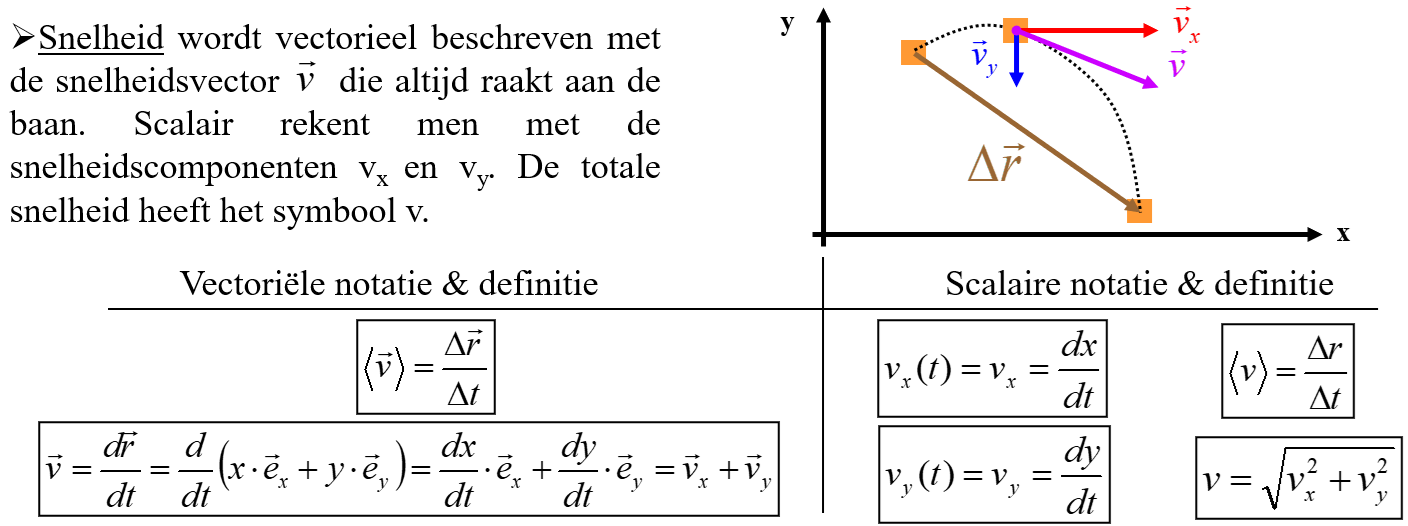
\includegraphics[width=0.8\textwidth]{snelheid2D}

% \end{image}


\begin{definition}
	
De \textbf{snelheidsvector \(\vec{v}\)} van een bewegend punt wordt gedefinieerd als de afgeleide van de plaatsvector naar de tijd:

\[
\vec{v}(t) = \frac{d\vec{r}(t)}{dt},
\]

en kan worden opgesplits in snelheidscomponenten \(v_x\) en \(v_y\):

\[
	\vec{v} = \frac{d\vec{r}}{dt} = \frac{d}{dt}(x \cdot \vec{e}_x + y \cdot \vec{e}_y) = \frac{dx}{dt} \cdot \vec{e}_x + \frac{dy}{dt} \cdot \vec{e}_y = \vec{v}_x + \vec{v}_y
\]
De grootte van de totale snelheid wordt genoteerd met het symbool \(v\) en is gelijk aan 
\[
v = \| \vec{v}\| = \sqrt{(\vec{v}_x)^2 + (\vec{v}_y)^2}
\]

\begin{image}[0.5\textwidth]
	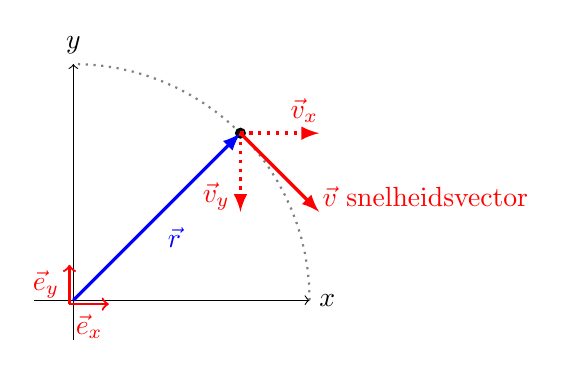
\begin{tikzpicture}
		\draw[->] (-0.5,0) -- (3,0) node[right] {$x$};
		\draw[->] (0,-0.5) -- (0,3) node[above] {$y$};
		\coordinate (O) at (0,0);

		\pgfmathsetmacro{\r}{3}       
		\pgfmathsetmacro{\ang}{45} 

		\coordinate (A) at (\ang :\r);
		\coordinate (X) at (\r*cos{\ang},0);
		\coordinate (Y) at (0,\r*sin{\ang});

		\draw[thick, gray, dotted, domain=0:90] plot ({\r*cos(\x)}, {\r*sin(\x)});

	
		\fill (A) circle (2pt);
	
		\draw[->, very thick, blue, -latex] (O) -- (A) node[midway, below right] { $\vec{r}$};
		% \draw[->, very thick, dashed, blue] (O) -- (X) node[midway, below] {$\vec{r}_x$};
		% \draw[->, very thick, dashed, blue] (O) -- (Y) node[midway, right] {$\vec{r}_y$};
		% \draw[thick, dotted, blue] (Y) -- (A) -- (X);
		
		
		\draw[->, very thick, red, -latex] 			(A) --++ (1, -1) node[pos=0.8, right, xshift=3pt]{ $\vec{v}$ snelheidsvector};
		\draw[->, very thick, red, dotted, -latex] 	(A) --++ (1, 0) node[midway, above right] { $\vec{v}_x$};
		\draw[->, very thick, red, dotted, -latex] 	(A) --++ (0, -1) node[pos=0.8, left ] { $\vec{v}_y$};


		\draw[->, thick, red, transform canvas={shift={(-0.05,-0.05)}}] (O) -- (0.5,0) node[midway, below] {$\vec{e}_x$};
		\draw[->, thick, red, transform canvas={shift={(-0.05,-0.05)}}] (O) -- (0,0.5) node[midway, left] {$\vec{e}_y$};
	\end{tikzpicture}
\end{image}
\captionof{figure}{De snelheidsvector \(\vec{v}\)}
	

\end{definition}

De snelheid werd gedefinieerd als afgeleide van de plaatsfunctie.
Uit de wiskunde weten we dat de afgeleide overeenkomt met de rico van de raaklijn. 
In de volgende eigenschap van de snelheidsvector komt dit fysisch tot uiting. 

\begin{theorem}
De snelheidsvector is altijd rakend aan de baan.

\begin{image}[0.4\textwidth]
	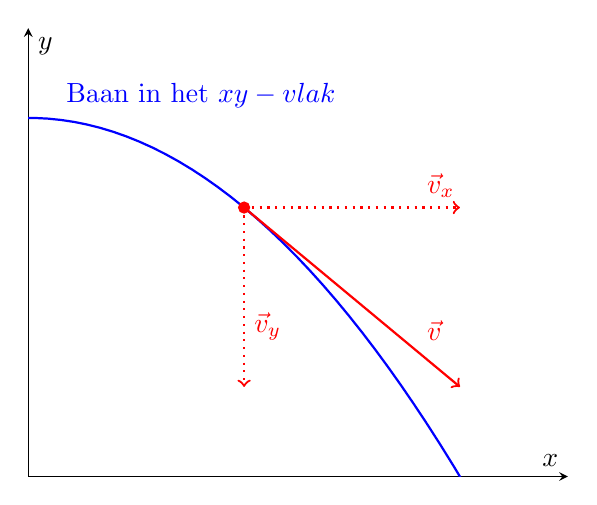
\begin{tikzpicture}
		\begin{axis}[
			axis lines=middle,
			xlabel={$x$},
			ylabel={$y$},
			ticks=none,        % removes all tick marks
			xmin=0, xmax=2.5,
			ymin=0, ymax=2.5,
			% grid=both,
			% minor tick num=1
		]
		\addplot[
			domain=-3:3, 
			samples=100, 
			thick, 
			blue
		]{-0.5*(x^2) + 2};
		% node[pos=0.3, above]{De baan in het \(xy-vlak\)};
	
		\node[blue, above] at (axis cs:0.8, 2) {Baan in het \(xy-vlak\)};
	
	
		\addplot[only marks, mark=*, mark size =2pt, red] coordinates {(1, 1.5)};
	
		\draw[->, thick, red] 
		(axis cs:1,1.5) -- (axis cs:2,0.5)
		node[pos=0.8, above right]{\(\vec{v}\)};
	
		\draw[->, thick, dotted, red] 
		(axis cs:1,1.5) -- (axis cs:2,1.5)
		node[pos=0.8, above right]{\(\vec{v}_x\)};
	
		\draw[->, thick, dotted, red] 
		(axis cs:1,1.5) -- (axis cs:1,0.5)
		node[pos=0.8, above right]{\(\vec{v}_y\)};
	
	
		\end{axis}
	
	\end{tikzpicture}
	\end{image}
	\captionof{figure}{De snelheidsvector is rakend aan de baan.}

\end{theorem}
	\begin{expandable}{proof}{}
	We kunnen dit bewijzen met de kettingregel, toegepast op de functie $y(t)=y(x(t))$.
	\begin{eqnarray*}
	 \frac{dy}{dt}=\frac{dy}{dx}\frac{dx}{dt}\Leftrightarrow\frac{dy}{dx}=\frac{\frac{dy}{dt}}{\frac{dx}{dt}}=\frac{v_y}{v_x}
	\end{eqnarray*}
	Inderdaad, $\frac{dy}{dx}$ is de helling van de baan en deze valt samen met de helling die de snelheidsvector maakt $\frac{v_y}{v_x}$.
\end{expandable}



% \subsection{Vectoriële notatie \& definitie}
% \[
% \langle \vec{v} \rangle = \frac{\Delta \vec{r}}{\Delta t}
% \]




% DIT KOMT UIT DE SLIDES VAN VINCENT 
% \subsection{Scalaire notatie \& definitie}
% \[
% v_x(t) = v_x = \frac{dx}{dt}
% \]
% \[
% v_y(t) = v_y = \frac{dy}{dt}
% \]
% \[
% \langle v \rangle = \frac{\Delta r}{\Delta t}
% \]
% \[
% v = \sqrt{(\vec{v}_x)^2 + (\vec{v}_y)^2}
% \]

	
\end{document}